\documentclass{my_paper}
\usepackage{ctex}
\usepackage[textwidth=444bp,vmargin=2.5cm]{geometry}%设置页边距
\usepackage{array} %主要是增加列样式选项
\usepackage[dvipsnames]{xcolor}%颜色宏包
\usepackage{graphicx}%图片宏包
\usepackage{amsmath}%公式宏包
\usepackage[T1]{fontenc}    
\usepackage{newtxtext, newtxmath}  %两种使用Times New Roman 字体的方法
\usepackage{subfigure}
\usepackage{tabularx, booktabs} %% Load packages that you use
\usepackage{multirow} %跨行处理
\usepackage{rotating}%横向表格
\usepackage{diagbox}%斜线划分表头

\usepackage { gensymb }
% 打°符号\degree
\usepackage{framed}
\usepackage{listings}
% 代码
\usepackage{color} %red, green, blue, yellow, cyan, magenta, black, white
\usepackage[numbered,framed]{matlab-prettifier}%matlab 代码高亮
\usepackage{mdframed}%另一个边框
% matlab代码样式,使用方法为:
% \lstinputlisting[style=Matlab-editor,linewidth=\textwidth]{code.m}
% 或:
% \begin{lstlisting}[style=matlab-prettifier]
%     %code
% \end{lstlisting}
\renewenvironment{framed}[1][\hsize]
  {\MakeFramed{\hsize#1\advance\hsize-\width \FrameRestore}}%
  {\endMakeFramed}
%   修正framed环境,使之可以变长,用法:
%   \begin{framed}[1.2/textwidth]...

\usepackage{hologo}
\usepackage{gbt7714}
\bibliographystyle{gbt7714-numerical}
% 采用国标参考文献引用
\newcommand{\lunwenbiaoti}{\fontsize{15.75pt}{0}\heiti 基于熵权法的企业供应链调度模型}
\newcommand{\zhaiyao}{\fontsize{14pt}{0}\heiti 摘要}
    
\begin{document}

\lstdefinestyle{python_style}{
 columns=fixed,
 numbers=left,                                        % 在左侧显示行号
 numberstyle=\tiny\color{gray},                       % 设定行号格式
 frame=trbl,                                        % 单线背景边框
 breaklines=true,                                     % 设定LaTeX对过长的代码行进行自动换行
 keywordstyle=\color[RGB]{40,40,255},                 % 设定关键字颜色
 numberstyle=\footnotesize\color{darkgray},
 commentstyle=\it\color[RGB]{0,96,96},                % 设置代码注释的格式
 stringstyle=\rmfamily\slshape\color[RGB]{128,0,0},   % 设置字符串格式
 showstringspaces=false,                              % 不显示字符串中的空格
 language=python,                                        % 设置语言
 basicstyle=\linespread{1.0}\fontsize{10bp}{10bp}\selectfont\ttfamily,                      % 字体字号
 %lineskip=10bp,
 %baselinestretch=1,
}
\newpage
\begin{center}
\lunwenbiaoti

\vspace{2ex}
\zhaiyao
\end{center}

企业要正常生产的前提条件是与供货商,转运商充分协调,根据各自特点进行原料订购和物资生产,以保证正常运作。本文从不同角度列出供应商的重要因素,并利用熵权法确定这些因素的权重,选出50家重要供应商,随后利用线性回归预测和单目标规划,确定了企业原料订购和物资转运的方案。对于减少原料体积和产能上限提升的情况,也对原有方案进行调整,以适应新的需求。

针对第一问,为了能够筛选出重要的供应商,我们提出了一种基于熵权法的打分模型,以履约执行性、供货稳定性、供货产能、签约存续性和库存持续性五个指标作为评判标准。最终全面的筛选出50家重要的供应商。

我们对问题二提出解决方案。首先基于问题一的结果,评估出供应商的供货能力,并确定供应商的数目。其次对企业保障库存和生产的需求以及转运过程中的损耗做出估计,确定了每周订购的原料总额。此后对供应商的供货量做线性预测,得到未来24周内的预估供货量,以此作为分配订单的指标。使用历史订单履约情况,对供应商交货的风险进行量化评估。

对于订购原料的指派转运商问题,列出最优化目标为装配产出最多的原料,针对供应商的分配关系,借鉴背包问题的解决思路来求解最优值。并提出了基于订购方案可实现度和转运量占用率的订购转运方案评价指标。

针对问题三,我们在选择重要供应商的过程中添加了类别优势,并对重要供应商进行重新选择。随后使用原有模型计算订购和转运方案,并比较了改变前后资金成本和仓储成本的变化情况。

针对问题四,我们合理扩大了供应商的最大供给能力限制,并求解了在此条件下企业每周产量的提高情况。
\begin{guanjianci}
 熵权法 \quad 线性预测 \quad 单目标规划
\end{guanjianci}

%----------- 正文 ----------
%----------- 一、问题重述 ----------
\newpage
\section{一、问题重述}

\subsection{问题背景}

一企业使用A、B、C三种可相互替代的原料生产某种建筑和装饰板材。在生产过程中,需要及时向供应商订购物资,并且指派转运商进行转运。由于原材料的特殊性,供应商
不能保证严格按订货量供货,实际供货量可能多于或少于订货量。且转运商在转运过程中可能导致原材料的损耗,不同的转运商具有不同的损耗率。

为了维持生产所需,企业应该尽量保持不少于两周的生产备货量,在这一系列条件下,我们需要基于材料所给数据,制定企业调度供应商以及转运商的策略。

\subsection{问题重述}
经过分析整理,我们需要解决以下问题:
\begin{enumerate}
    \item 对402家供应商的订货以及供货情况进行分析,建立保障企业生产重要性的数学模型,在所给的供应商中选出50个最重要的供应商,在论文中列出结果。
    \item 在问题一的基础上,估计满足企业生产需求所需的供应商数目,对于这些供应商而言,制定最经济的订购方案以及损耗最少的转运方案,以指定格式输出到附件中。
    \item 为了压缩企业的仓储成本,计划尽量多的采购A类原材料和尽量少的采购C类原材料,同时希望企业的转运损耗尽可能小。就此确定新的采购方案,并且分析新采购方案的实施效果。
    \item 若企业经过技术改造后,具有提高产能的潜力,根据供应商和转运商的实际情况,确定每周的产能提高情况,并给出订购和转运的方案。
\end{enumerate}
\section{二、问题分析}
\subsection{问题一的分析}

针对问题一,需要确定402家供应商中最重要的50家。为此,需要由附件中的企业订货数量和供应商的供货量之间的关系进行判断。由于供货的特殊性,供货与订货数量不能完全保持一致,若供货不及时,可能带来原料缺口,影响企业的生产过程。

与此同时,不同供应商之间的供应能力也有较大差异,部分供应商倾向于连续供货,而部分倾向于集中供货。我们需要将指标量化后,综合赋予权重,对每家供应商进行打分,最终比较出最重要的50家供应商。

\subsection{问题二的分析}

针对问题二,我们需要在问题一的基础上选出足以满足生产要求的供应商数目,并对企业向供应商的订单情况进行组合,给出各个供应商的每周订单。并且根据转运商的损耗率指标来确定转运商的分配工作。为了解决第一小问,需要结合前面问题的结果来处理,并估计所得产能是否能满足生产所需。

第二小问,我们需要给出具体的分配方案,需要从库存储备,供应商生产能力变动,供应商交付特点等因素来考虑。为此,需要制定计划保持企业库存,对未来供应商的能力变化做预测,并考虑供应商的历史订单执行情况。

针对第三小问,在得到未来24周内的企业订单数量后,指派八家企业到不同供货商运送货物,在满足所有送货需求的同时,保证损耗率保持在低水平。

\subsection{问题三的分析}

在问题三中,需要压缩企业的库存成本,以降本增效。为此我们在选择供应商时应当优先考虑C类原料的供应商,为此在第一问的基础上添加原料优势因子,在加以权重判断,订购方案和转运方案的过程保持不变。

\subsection{问题四的分析}

在问题四中,企业具有了扩大产量的能力,因此需要扩大供应链的供给,以提高企业产能。
%----------- 三、模型假设 ----------
\section{三、模型假设}
%使用代码片段:、jiashe%
\begin{enumerate}
    \item 假设供应商能够在一周内交付订单。
    
    \textbf{原因:}由于周转时间等因素难以把控,不同供应商的调度管理水平不同,因此认为供应商能够在一周内交付订单,便于模型的建立。

    \item 假设第241周时库存为0。
    
    \textbf{原因:}该假设具有两方面的原因,其一:经由分析,前240周的所有供应商平均供应量不足应对每周生产,可能在这一过程中持续消耗库存。其次,企业库存难以确定,该假设有助于简化问题。
    
\end{enumerate}

%----------- 四、符号说明 ----------
\section{四、符号说明}
%使用三线表格最好~

\subsection{符号说明}
以下是本文使用的符号以及含义:
\begin{table}[h]%htbp表示的意思是latex会尽量满足排在前面的浮动格式,就是h-t-b-p这个顺序,让排版的效果尽量好。
    \centering
    \begin{tabular}{p{2.0cm}<{\centering}p{9.0cm}<{\centering}p{2.0cm}<{\centering}}
 %指定单元格宽度, 并且水平居中。
    \hline
    符号 & 说明 & 单位 \\ %换行 
    \hline
    $R$ & 企业订货量 &  $m^3$\\
    $S$ & 供应商供货量 &  $m^3$\\
    $b$ & 订单空白 &  $/$\\
    $c$ & 供求评分 &  $/$\\
    $i$ & 周数 &  周\\
    $j$ & 供应商编号 &  $/$\\
    $k$ & 转运商编号 &  $/$\\
    $d$ & 连续供货周数 &  周\\
    $M$ & 原料种类 &  $/$\\
    $\alpha$ & 产出系数 &  $/$\\
    $h$ & 原料库存 &  $m^3$\\
    $f$ & 评价函数 &  $/$\\
    $A$ & 供货产能 &  $m^3$\\
    $L$ & 运输损耗率 &  $/$\\
    $T$ & 周转运量 &  $m^3$\\
    $N$ & 企业需求 &  $m^3$\\
    $\eta$ & 履约比例 &  $/$\\
    \hline
    \end{tabular}
\end{table}
\newpage
%----------- 五、模型的建立与求解 ----------
\section{五、模型的建立与求解}

以下将对提出的四个问题进行建模求解。

\subsection{重要供应商筛选模型}
为了能够筛选出重要的供应商,我们提出了一种基于熵权法的打分模型,以履约执行性、供货稳定性、供货产能、签约存续性和库存持续性五个指标作为评判标准。最终筛选出50家重要的供应商。
\subsubsection{模型建立}
经过分析和思考,我们列出五个反应供应商情况的重要指标,综合了每周和长期的订单交付情况。这五个指标综合反映了供应商的特点,较为全面综合了局部与全局的信息。

\begin{enumerate}
    \item 履约执行性 $a_1$
    
    在供应链管理的过程中,风险管理\cite{1}是非常重要的环节,事关企业的生产计划能否按需完成。在题目的条件中,我们不能获悉供应商的财务报表、人事构成等情况,但是可以通过企业的订货量$R$和供应商的供货量$S$之间的关系来分析企业的履约情况,也就是履约执行性$a_1$。该指标判断了供应商在有订单的条件下,执行订单的总体情况。要量化计算履约执行性,我们首先需要引入两个指标:订单空白$b_{ij}$和供求评分$c_{ij}$。订单空白是个二值变量,用于标记某供应商在某周是否有订单;供求评分$c_{ij}$是一个分段函数,用于量化估计供应与订单量的相对大小。二者的计算公式如下所示:
    \begin{equation}
    b_{ij} = \begin{cases}
        0&,R_{ij}=0\\
        1&,R_{ij}\neq 0\\
    \end{cases}
    \label{bij}
    \end{equation}
    \begin{equation}
    c_{ij}=\begin{cases}
        0,&R_{ij}>S_{ij}\\
        1,&R_{ij}=S_{ij}\\
        0.8,&R_{ij}<S_{ij}\\
    \end{cases}
    \label{cij}
    \end{equation}
    ,其中$R$和$S$分别代表企业的订货量和供应商的供货量。上述公式中$i$代表周数,$j$代表供应商的编号,下同。
    
    $c$的意义在于判断订单的执行情况,最理想的条件下,企业发出订单,在一周内供应商能够按约定量交付,则此时量化评分为1;若供应商不能够按约执行的话,分为两种情况进行考虑:一种是供大于求,此时虽然没有按约执行,但是充实了企业的备用库存,结果不算差,故量化评分为$0.8$。另一种是供不应求,此时企业消耗库存以填补原料缺口,可能导致库存消耗甚至是影响产量的问题。
    
    在得到两个中间变量后,便可给出履约情况的计算式:
    \begin{equation}
    a_{j1}=\frac{\sum\limits^n_{i=1}c_{ij}}{\sum\limits^n_{i=1}b_{ij}}
    \label{aj1}
    \end{equation}
    ,其中$n$为附件数据中所给的周数。$a_i$的意义在于量化统计供应商在每周内的履约情况。对于那些没有在一周内按数量交付的供应商,该评分的数值较低,而如果一家供应商能够准时供货,则该指标数值就较大。

    \item 供货稳定性 $a_2$
    
    选取两个供应商的每周供货情况,绘制成折线图,如图(\ref{11})所示。
    \begin{figure}[htbp]
        \centering  %居中
        \subfigure[S005]{   %第一张子图
        \begin{minipage}{\textwidth}%大小总和超过textwidth则自动换行
        \centering    %子图居中
        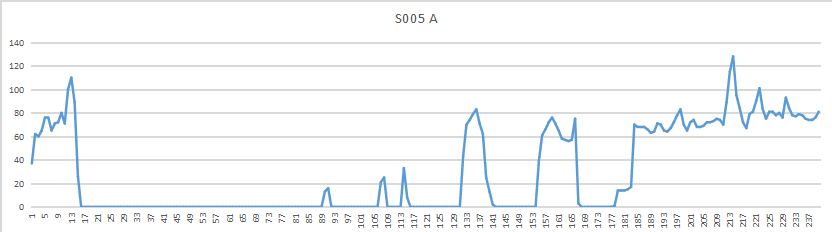
\includegraphics[width=\textwidth]{11005.png}  %设置图片的输出大小倍数,这里是0.5倍大小输出
        \end{minipage}
        }\\
        \subfigure[S007]{ %第二张子图
        \begin{minipage}{\textwidth}
        \centering    %子图居中
        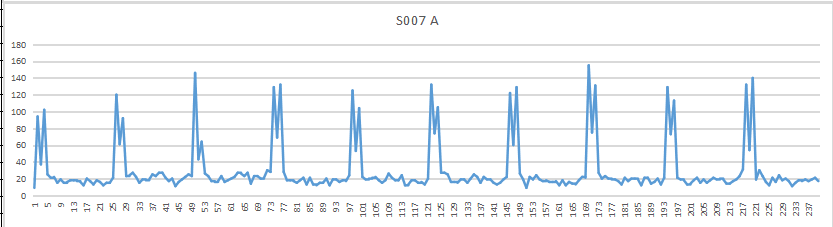
\includegraphics[width=\textwidth]{11007.png}%以pic.jpg的0.5倍大小输出
        \end{minipage}
        }
        注:横轴为周数单位为周,纵轴为供货量单位为$m^3$
    
        \caption{不同供应商的供货情况}    %大图名称
        \label{11}    %图片引用标记
    \end{figure}
    \newpage
    可见供应商由于各种原因,可能不具有连续供应的能力,导致一段时间内企业不能收到原材料。为此,提出供货稳定性这一指标$a_2$,用于统计供应商能够连续供货的情况。其计算方法为统计订单和供货量均大于0的最大连续天数$d$,计算方法如下:
    \begin{equation}
    d_i = \begin{cases}
        d_{i-1}+1,&R_i>0 \quad\&\quad S_i>0\\
        0, & else
    \end{cases}
    \label{d}
    \end{equation}
    ,其中$d_0=0$,对序列进行计算后,令其中的最大值为$a_2$,即:
    \begin{equation}
    a_{j2}=\underset{i}{argmax}\quad d_{ij}
    \label{aj2}
    \end{equation}
    对于供应商而言,具有较高的$a_2$数值意味着具有更好的连续供货的能力,以满足连续的生产需求,更有利于判断其生产的规律性。而具有较低数值的企业可能会有较大供应波动,导致不合理的订货情况。

    \item 供货产能 $a_3$
    
    观察附件中数据可知,不同供应商之间的供应能力也有较大差异,表现在每周的供货数量的平均值上有一定区别。之所以不使用最大值来评估供货商的供应能力,是因为某天内供应商的大量出货可能是由于订单数目的增多,不能够全面反映出供应商的原料出产水平。此外,供应商可能会提供A、B、C三种原料中的一种,不同原料的出品率有所不同,因此需要衡量企业最终产出的数量。考虑到企业每周的生产量达到了万立方米级别,因此供应商的产量不能太低,否则导致调度配合过程中成本上升。综合上述分析,提出供货产能$a_3$的计算方法:
    \begin{equation}
    a_{j3}=\frac{\sum\limits^n_{i=1} S_i}{n}\cdot \alpha
    \label{aj3}
    \end{equation}
    ,$\alpha$是产出系数,同原料种类$M_j$的不同而变化:
    $$\alpha=\begin{cases}
        \frac{1}{0.6} ,& M_j=A\\
        \frac{1}{0.66} ,& M_j=B\\
        \frac{1}{0.72} ,& M_j=C\\
    \end{cases}$$

    \item 签约存续性 $a_4$
    
    在历史的订单数据中,企业已经同供应商合作240周的时间,这段时间中供应商若能同企业配合良好,企业便有更高的概率向这一企业订购材料;而反之若双方合作不愉快,企业便不愿意再订购,长期上看便是具有较少的交货量。经过上述分析,给出签约存续性$a_{4}$的计算式:
    \begin{equation}
    a_{j4}=\frac{\sum\limits^n_{i=1}b_{ij}}{n}
    \label{aj4}
    \end{equation}
    ,其中$b_{ij}$已经由式(\ref{bij})给出,表示的是某周是否交付原料。

    \item 库存持续性 $a_5$
    
    如背景中所述,企业在规划生产活动时,会预留两周的原料储备,以应对不能即使供应的情况,这部分库存常被称作是安全库存\cite{1}。安全库存的概念是就企业整体的生产而言,但是我们可以就整体和局部的关系来看,如果企业的每个供应商都能够保证订单交付的情况能满足安全库存,则企业的安全库存无虞。
    
    在这一前提条件下,我们认为企业向某个供应商定下的订单是基于库存和生产需求来确定的,若某周供应商的库存不能满足未来两周的订单要求,则认为是“缺口周”。以附件一中S66供应商W001-W006的数据来分析可得下表:
    \begin{table}[ht]

    \centering
    \caption{以S66供应商为例分析缺口周情况表}
    \begin{tabular}{c|ccccccc}
    \toprule
    周数      & W001 & W002 & W003 & W004 & W005 & W005 & W006 \\\midrule
订货量     & 1    & 0    & 1    & 0    & 0    & 0    & 3    \\
供货量     & 2    & 0    & 1    & 0    & 0    & 0    & 4    \\
仓库剩余原料量 & 1    & 1    & 1    & 1    & 1    & 1    & 2    \\
未来两周订货量 & 1    & 1    & 0    & 0    & 3    & 3    & 3    \\
是否为缺口   & 否    & 否    & 否    & 否    & 是    & 是    & 是\\
    \bottomrule
      \end{tabular}
    
    \label{label}
      \end{table}
    
    我们提出的库存持续性$a_5$这一指标即统计了缺口时长。首先以递归形式给出原料库存$h$的计算公式:
    \begin{equation}
    h_i=h_{i-1}+R_i-S_i
    \label{hi}
    \end{equation}
    ,其中$h_0=0$,只需遍历订单和供应量列表即可获得库存的情况,在此基础上判断与未来两周的需求可以统计出$a_5$:
    \begin{equation}
    a_{j5} = |\{ h_{ij} |\forall 1\leq i \leq n-2 \quad h_{ij}\geq R_{i+1,j}+R_{i+2,j}\}|
    \label{aj5}
    \end{equation}
    
\end{enumerate}

在分析总结出履约执行性、供货稳定性、供货产能、签约存续性和库存持续性这五个重要的因素之后,需要对这些因素进行归一化处理,以判断其相对的重要程度。在众多方法如AHP主成分分析法\cite{2},熵权法\cite{3},主观赋权法之间,我们使用熵权法来衡量指标之间的重要程度。由于上述五个指标量纲不一致,需要对数据进行归一化处理,计算式如下:
\begin{equation}
a_{ij}=\frac{a_{ij}-min(a_i)}{max(a_i)-min(a_i)}
\label{aij}
\end{equation}

在归一化之后,使用熵权法计算各个指标应当配比的权重,其基本思想是根据指标的变化幅度来赋予权重。熵权法的计算过程如下所示:

\begin{align}
    p_{ij} &= \frac{a_{ij}}{\sum\limits^n_{i=1}a_{ij}}\\
    \label{p}
    e_j &= -\frac{1}{\ln n}\sum\limits^n_{i=1}p_{ij}\\
    \label{ej}
    g_j &= 1-e_j\\
    % \label{gj}
    w_j &= \frac{g_i}{\sum\limits^m_{j=1}g_j}
    \label{dw}
    \end{align}
    式(\ref{p})利用各个指标出现的概率$p$计算熵值,并且在式(\ref{dw})中计算各项指标的权重$w_{i}$。该方法由数据自身给出结果,较为客观有效。

综合上述成果,在得到各项指标的权重后,便可得出每家供应商的打分函数$f$:
\begin{equation}
f_j = w_1\cdot a_{j1}+w_2\cdot a_{j2}+w_3\cdot a_{j3}+w_4\cdot a_{j4}+w_5\cdot a_{j5}
\label{fj}
\end{equation}
其中各个指标的计算方法和含义如下,分别已经在式(\ref{aj1},\ref{aj2},\ref{aj3},\ref{aj4},\ref{aj5})给出:
$$\begin{cases}
    a_{j1}&=\frac{\sum\limits^n_{i=1}c_{ij}}{\sum\limits^n_{i=1}b_{ij}}\\
    a_{j2}&=\underset{i}{argmax}\quad d_{ij}\\
    a_{j3}&=\frac{\sum\limits^n_{i=1} S_i}{n}\cdot \alpha\\
    a_{j4}&=\frac{\sum\limits^n_{i=1}b_{ij}}{n}\\
    a_{j5}& = |\{ h_{ij} |\forall 1\leq i \leq n-2 \quad h_{ij}\geq R_{i+1,j}+R_{i+2,j}\}|\\
\end{cases}$$


\subsubsection{模型求解}
经过模型求解后,最终得出了基于402家企业的评分函数:
$$f_j = 0.0326\cdot a_{j1}+0.1638\cdot a_{j2}+0.5289\cdot a_{j3}+0.0610\cdot a_{j4}+0.2138\cdot a_{j5}$$
根据数据分析可知,在五个指标间供货产能$a_{3}$的权重较大(0.5289),说明其波动的情况较为明显,库存持续性次之,而履约执行性$a_1$的权重最小(0.0326),说明其变化幅度不大。

对402家供应商进行打分后,输出为以下结果:
\begin{table}[hbt]
\centering
\caption{50家重要供应商的编号以及对应评分}
\begin{tabular}{cc|cc|cc}
\toprule
编号  & 评分          & 编号  & 评分       & 编号  & 评分       \\\midrule
\textbf{229} & 0.050409816 & \textbf{352} & 0.014769 & \textbf{294} & 0.006183 \\
\textbf{361} & 0.038236735 & \textbf{143} & 0.014006 & \textbf{80 } & 0.005943 \\
\textbf{140} & 0.037887796 & \textbf{348} & 0.013749 & \textbf{367} & 0.005829 \\
\textbf{108} & 0.03289724  & \textbf{374} & 0.011999 & \textbf{55 } & 0.005678 \\
\textbf{282} & 0.03120258  & \textbf{307} & 0.011866 & \textbf{338} & 0.005215 \\
\textbf{329} & 0.026648442 & \textbf{201} & 0.011784 & \textbf{189} & 0.005142 \\
\textbf{275} & 0.026248195 & \textbf{395} & 0.011046 & \textbf{346} & 0.004442 \\
\textbf{151} & 0.025303675 & \textbf{247} & 0.010991 & \textbf{266} & 0.004436 \\
\textbf{340} & 0.023824746 & \textbf{365} & 0.009996 & \textbf{123} & 0.004416 \\
\textbf{139} & 0.020588064 & \textbf{31 } & 0.009758 & \textbf{5  } & 0.00436  \\
\textbf{356} & 0.019533442 & \textbf{284} & 0.007859 & \textbf{7  } & 0.003846 \\
\textbf{306} & 0.019469278 & \textbf{37 } & 0.007712 & \textbf{76 } & 0.003613 \\
\textbf{308} & 0.019217359 & \textbf{40 } & 0.007003 & \textbf{244} & 0.00354  \\
\textbf{268} & 0.019176436 & \textbf{218} & 0.006265 & \textbf{98 } & 0.003521 \\
\textbf{330} & 0.018571821 & \textbf{126} & 0.006251 & \textbf{273} & 0.003499 \\
\textbf{131} & 0.018529595 & \textbf{364} & 0.006247 & \textbf{86 } & 0.003362 \\
\textbf{194} & 0.015294734 &  &          & \textbf{67 } & 0.003291\\
\bottomrule
  \end{tabular}
\label{res1}
  \end{table}

为了直观展现分数的分布情况,我们又对所有供应商按分数从高到低的顺序进行排序,得到折线图(\ref{zx})。

\begin {figure}[h]
\centering % 居中显示
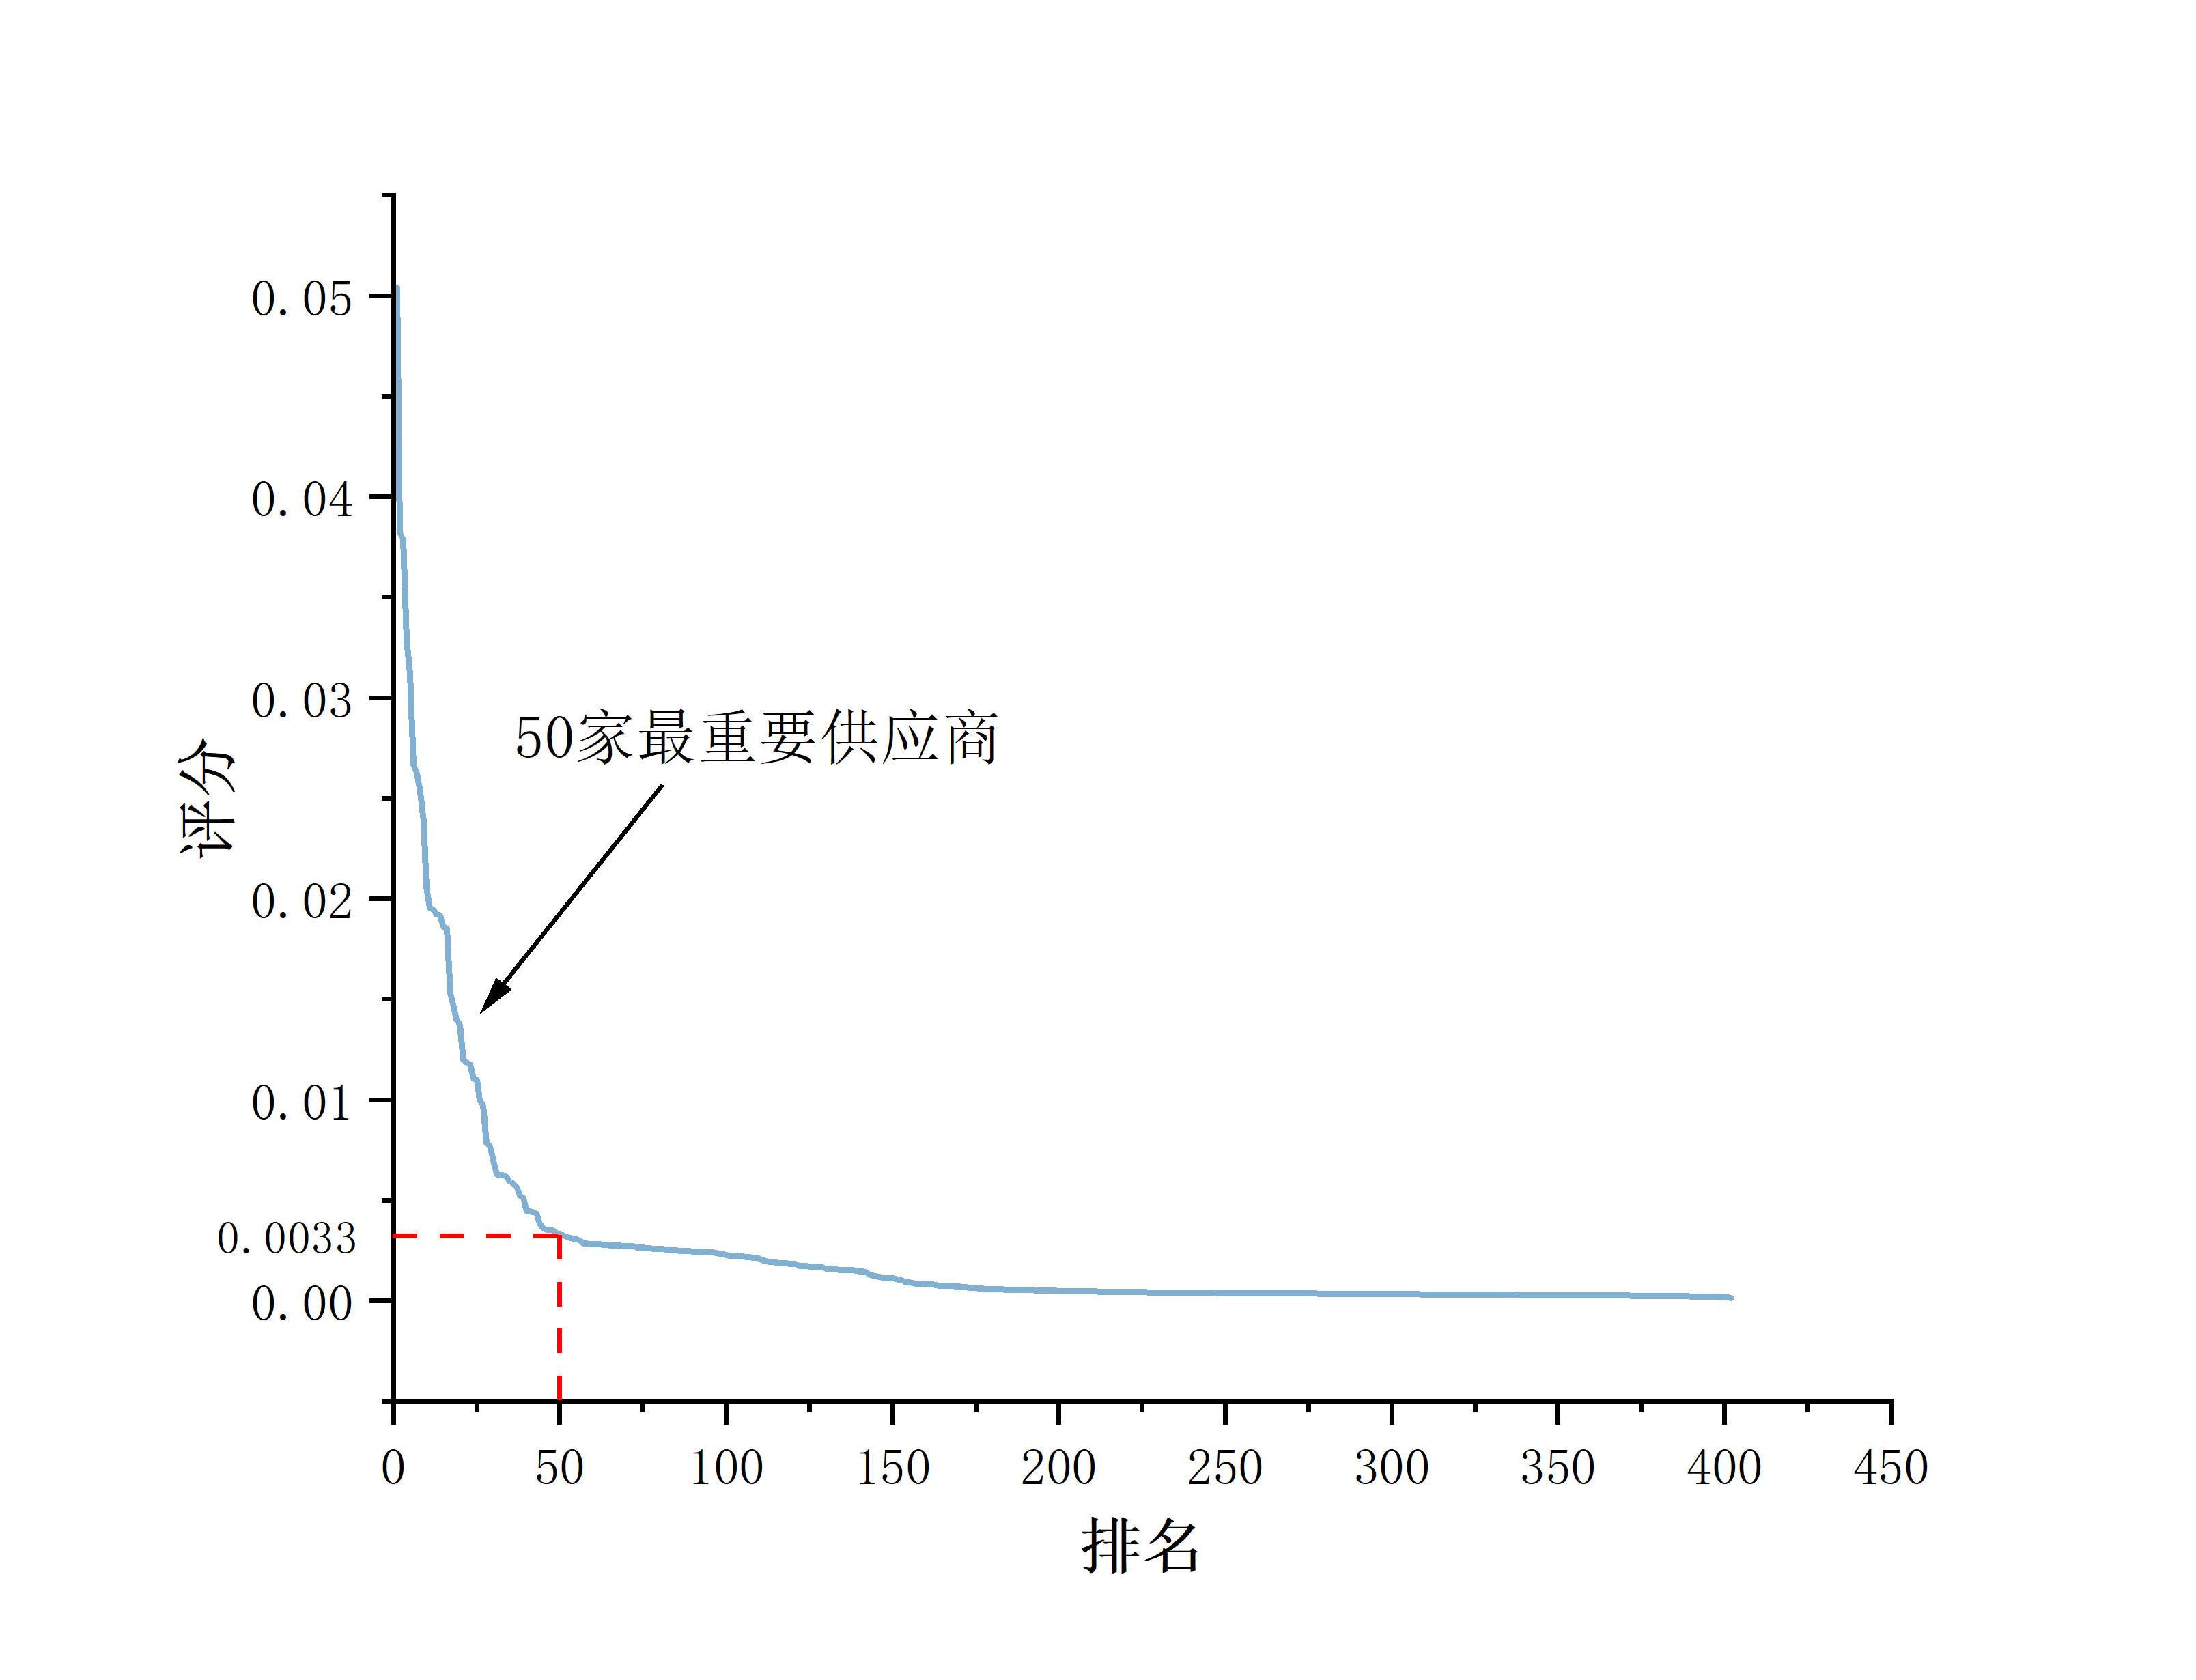
\includegraphics[width=\textwidth]{Graph1.jpg}
\caption{402家供应商的分数排名情况} % 标题
\label{zx}
\end {figure}

\newpage
可见前50位供应商占据了分数的绝大多数部分(68.1\%),呈现出优质供应商集中在头部的现象。这也佐证着选取评价函数的合理性,前50名供应商同后面的供应商形成了显著对比。

为了合理调配生产,我们随后又对供应商的供货种类进行了统计,得到饼图(\ref{bingtu})。
\begin {figure}[h]
\centering % 居中显示
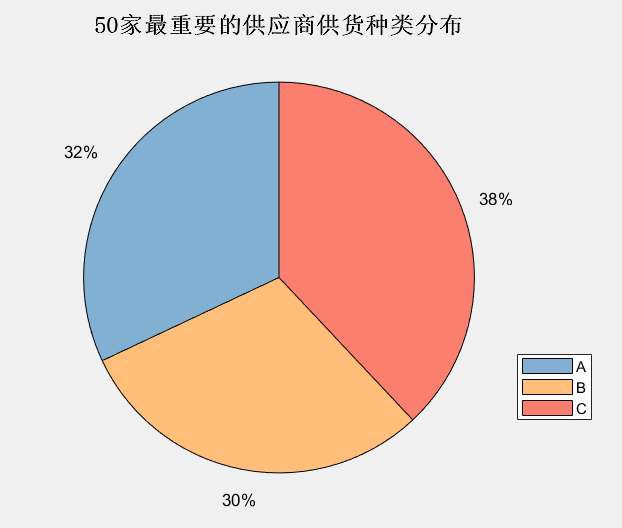
\includegraphics[width=0.6\textwidth]{bingtu.png}
\caption{50家评分最高供应商的材料种类分布} % 标题
\label{bingtu}
\end {figure}

\newpage
由图可知各个供应商呈现较为平衡的供货种类分布,对于后续订货分配以及调配过程带来的影响较小。

\subsection{基于背包算法的订购转运模型}
在该部分,我们将对问题二提出解决方案。首先基于问题一的结果,评估出供应商的供货能力,并确定供应商的数目。其次对供应商的供货量做线性预测,得到未来24周内的预估供货量,以此作为配额。使用历史订单履约情况,对供应商交货的风险进行量化评估。对于指派转运商问题,列出最优化目标为装配产出最多的原料。
\subsubsection{最佳供应商的数量确定}
经过5.1的分析,我们得出打分最高的50家供应商并认定为重要供应商。为了评估多少供应商能够满足生产需求,在不考虑供应风险的情况下,我们求取了重要供应商(50家)同所有供应商(402家)的周平均产出量。这一平均产出量将不同种类的原料同一处理,转化为供货产能,计算式如下:
\begin{equation}
    \begin{aligned}
        A &= \sum\limits^m_{j=1} a_{j3} \cdot n\\
          &= \sum\limits^m_{j=1}\sum\limits^n_{i=1} S_i\cdot \alpha\\
    \end{aligned}
\label{A}
\end{equation}
,其中$S$代表供应原料的数量,$n$代表周数,$m$代表供应商数目,
$\alpha$是产出系数,同原料种类$M_j$的不同而变化:
    $$\alpha=\begin{cases}
        \frac{1}{0.6} ,& M_j=A\\
        \frac{1}{0.66} ,& M_j=B\\
        \frac{1}{0.72} ,& M_j=C\\
    \end{cases}$$
% \newpage
经过计算得到下表:
\begin{table}[ht]
\centering
\caption{供应商平均周产出数量示意图}
\begin{tabular}{c|ccc}
\toprule
& 重要供应商   & 所有供应商   & 每周计划生产量 \\\midrule
平均周产出数量      & 26890   & 27778   & 28200   \\
占计划生产量的比例 & 95.36\% & 98.50\% & 100\%   \\
\bottomrule
  \end{tabular}
\label{label}
  \end{table}

可见即使是所有供应商的周平均产出也不能满足企业的每周计划生产量,但无论是重要供应商还是所有供应商,均能够满足$95\%$以上的产品需求。加之重要供应商所能生产的产品数量能够占到所有供应商的$96.8\%$所以在加大订单数量时,仅靠重要供应商也能满足所需。

此外,在5.1中所述的量化模型中综合考虑了长短周期下供货商的履约情况,更为全面的考虑到风险的可能性。在有关资料\cite{1}中指出,选择更少的供应商可以减少企业调度管理的成本,在需求一定时更少的供应商可以带来更大进货量,以得到效率的提升。

综合上述分析,我们认为选取50家重要供应商可以满足企业的生产要求,这些供应商的编号已经由表(\ref{res1})给出。

\subsubsection{订购方案计算}
在确定企业每周的需求前,需要考虑转运商在转运原料的过程中损消耗的数量。由于各家转运商的运送方式不同,导致损耗率因企业和时间而异。由于上述原因,我们利用均值,对整体转运损耗率$L_0$进行估计,给出以下计算式:
\begin{equation}
L_0 = \frac{\sum\limits^8_{i=1}\sum\limits^{240}_{j=1}l_{ij}}{\sum\limits^8_{i=1}\sum\limits^{240}_{j=1}E_{ij}}
\label{l0}
\end{equation}
,这里$l_{ij}$代表第$j$家转运商在第$i$周时转运的损耗率 ,$ E_{ij} $代表在该周是否转运货物,与周转运量$T$有关,下面给出计算式:
\begin{equation}
E_{ij} = \begin{cases}
    0 ,& T_{ij}=0\\
    1 ,& T_{ij}>0\\
\end{cases}
\label{eij}
\end{equation}

在获得总体损耗率之后,企业将确定其生产计划,以及库存情况。经过分析,企业在前240周总共收到的原材料均值不能满足每周的产能,故假设在前240周生产的不足之处均为消耗仓库原料余量。在理想情况下,未来的首周应当补充库存至满足两周生产的需求,随后几周都只需保障本周生产即可。考虑到损耗率的影响,给出企业总需求的计算式:

\begin{equation}
N_i = \begin{cases}
    \frac{2.84\times 10^4 \times 3 }{1-L_0}&,i=241 \\
    \frac{2.84\times 10^4 }{1-L_0}&,241<i\leq 264\\
\end{cases}
\label{ni}
\end{equation}

在得到企业每周需求后,需要确定每周的订购方案。也就是说企业每周的需求$N_i$应当分配到选定的50家供应商,故需要分析每家企业的供货能力,以及其履约情况。

观察供应商的年际变化数据可知,供货数据呈很强的周期性变化,每一年的同一周的数据往往非常相近,如图(\ref{zhouqi},\ref{zhouqi2})所示。为了体现这一特点的同时还掌握其年际变化趋势,可以使用线性拟合的方式对未来数据做出预测。

\begin {figure}[h]
\centering % 居中显示
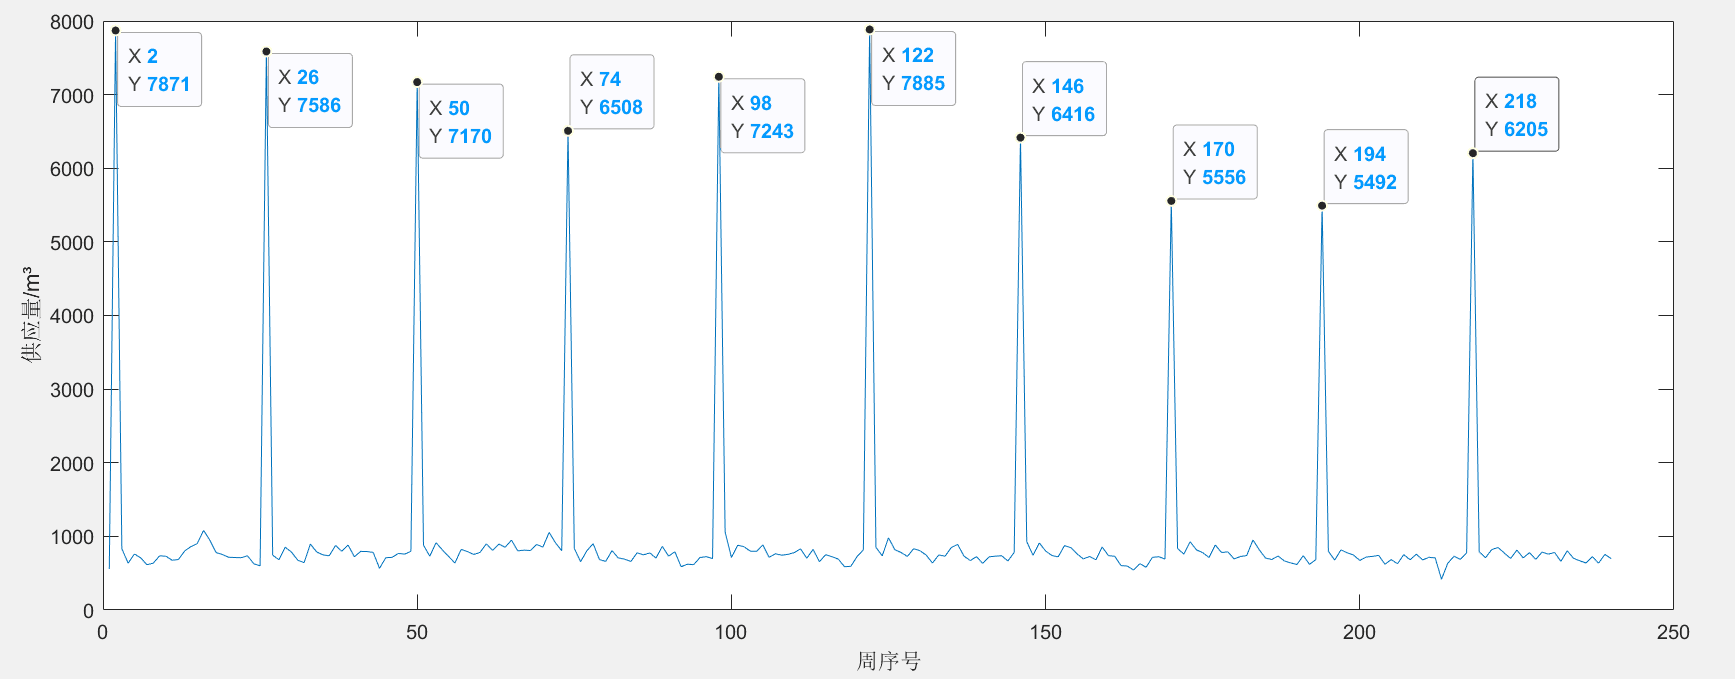
\includegraphics[width=\textwidth]{zhouqi.png}
\caption{S108 的供货情况分析} % 标题
\label{zhouqi}
\end {figure}

\begin {figure}[h]
\centering % 居中显示
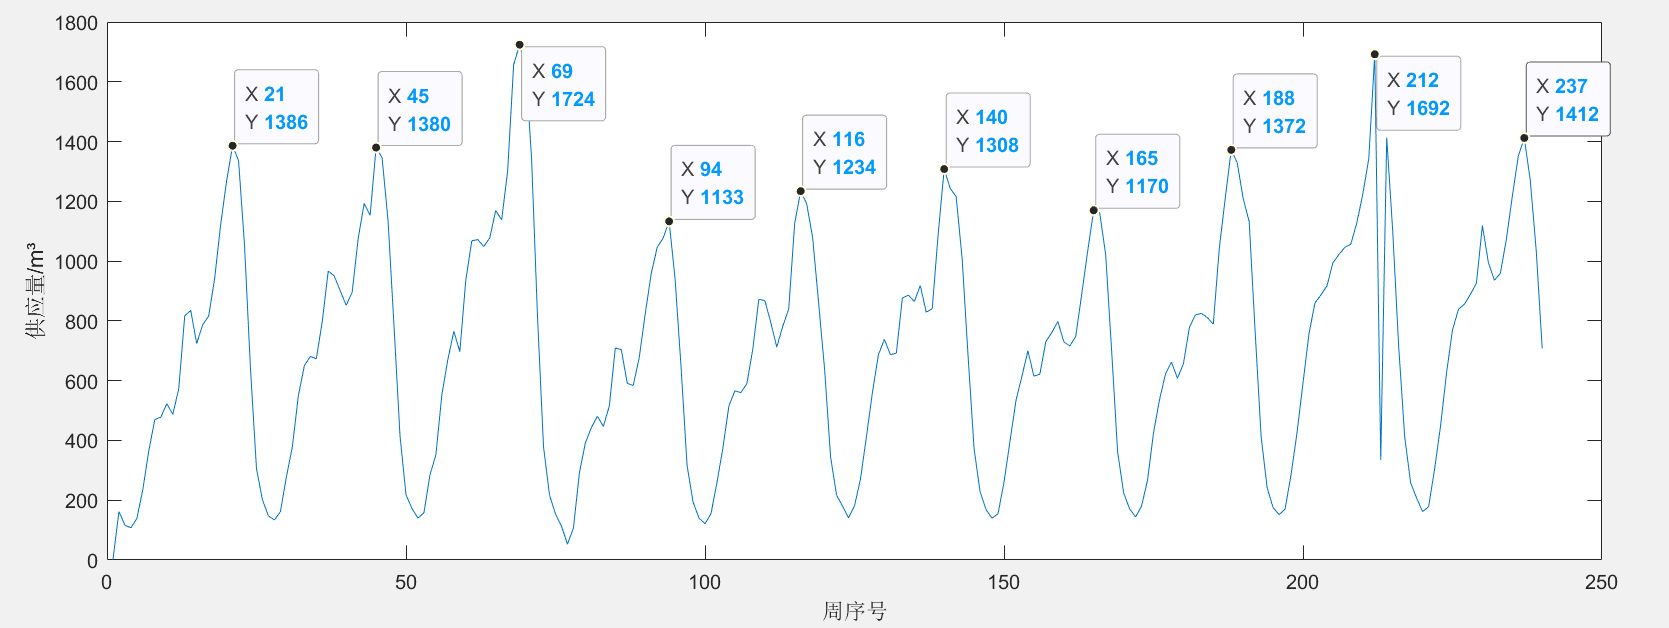
\includegraphics[width=\textwidth]{zhouqi2.png}
\caption{S282 的供货情况分析} % 标题
\label{zhouqi2}
\end {figure}
我们首先使用线性拟合的方式,对每一年(48周)中的同一周数据进行线性拟合,得出第六年该周的供货数量预测值$\hat{C}_{ij}$。这一预测值作用是估算由于年际变化而导致的供给能力变化,不同供应商的变化情况不同,掌握这一差异性有助于对订单进行分配。

随后估计供应商每周的供货情况,也就是判断其平均每周的履约比例$\eta$,给出计算式如下:

\begin{equation}
\eta = \frac{\sum\limits_{R_{ij}\neq 0} \frac{S_{ij}}{R_{ij}}}{|\{i|\forall 1\leq i\leq 240 \quad R_{ij}\neq 0 \}|}
\label{eta}
\end{equation}
,这一平均履约比例衡量了在有订单时供应商的交付数量,若供应商倾向于少交付,则利用这一平均比例可以适当增加订购数量,以获取足够的原材料。

在获得企业周需求$N_i$、供货量预测$C_{ij}$以及平均履约比$\eta$后便可对企业的进货需求进行订单分配。分配过程中需要考虑不同材料的消耗量不同,综合上述分析,我们给出以下计算式:
\begin{equation}
\hat{R_{ij}} = N_i\cdot \frac{C_{ij}}{\sum\limits^{50}_{j=1}C_{ij}\cdot \eta \cdot \alpha}
\label{rijr}
\end{equation}
,其中$\hat{R_{ij}}$代表第$i$周第$ j $家供应商的订货量($j=241,242,\cdots,264$)。相关参数的计算式已经由式(\ref{l0}-\ref{eta})给出:

$$L_0 = \frac{\sum\limits^8_{i=1}\sum\limits^{240}_{j=1}l_{ij}}{\sum\limits^8_{i=1}\sum\limits^{240}_{j=1}E_{ij}}$$
$$E_{ij} = \begin{cases}
    0 ,& T_{ij}=0\\
    1 ,& T_{ij}>0\\
\end{cases}$$
$$N_i = \begin{cases}
    \frac{2.84\times 10^4 \times 3 }{1-L_0}&,i=241 \\
    \frac{2.84\times 10^4 }{1-L_0}&,241<i\leq 264\\\end{cases}$$
$$\eta = \frac{\sum\limits_{R_{ij}\neq 0} \frac{S_{ij}}{R_{ij}}}{|\{i|\forall 1\leq i\leq 240 \quad R_{ij}\neq 0 \}|}$$


\newpage
\subsubsection{转运方案的计算}
与式(\ref{l0})的计算方法相似,首先对所有转运企业的运输损耗率$L_j$进行计算:
\begin{equation}
    L_j = \frac{\sum\limits^{240}_{j=1}l_{ij}}{\sum\limits^{240}_{j=1}E_{ij}}
\label{lj}
\end{equation}
$$E_{ij} = \begin{cases}
    0 ,& T_{ij}=0\\
    1 ,& T_{ij}>0\\
\end{cases}$$
在计算出各个转运商的平均损耗率后按照损耗率的大小进行排序,优先选择损耗率较小的供应商安排转运。由于有8家企业参与转运,每家企业的转运$T$量都达到$6000m^3$,足以满足转运量的峰值,而在仅供生产时会有转运商空缺。这样做的好处是在于优先保障了损耗小的转运商尽可能多运送原料,可以达到损耗最低的目标。

由于考虑到一个供应商尽量只由一个转运商来转运,转运商与供应商的组合问题可以转化为背包问题。转运商对于每个供应商而言只有两种状态,转运和不转运,利用决策变量$x^k_{ij}$来表示:
\begin{equation}
x^{k}_{ij} = \begin{cases}
    1,& \text{第i周装载第j个供应商的原料}\\
    0,& \text{第i周不装载第j个供应商的原料}\\
\end{cases}
\label{xij}
\end{equation}

对于所有转运商$k$而言,目的是转运尽可能多的货物数量,故列出其目标函数:
\begin{equation}
max \quad z^k_j = \sum\limits^{164}_{i=241} x^{k}_{ij}\cdot n_{ij} \cdot \alpha
\label{z}
\end{equation}
\begin{equation}
    s.t.\begin{cases}
        \sum\limits^{164}_{i=241} n_{ij}\cdot \leq 6000\\
        x^{k}_{ij} = 0,1 \\
    \end{cases}
\end{equation}

便可以顺次解出转运方案的最优解。

\subsubsection{问题求解}
针对订购方案的实现效果,我们提出订购方案可实现度$Q$来衡量。由于企业的订单量$C$同供货量$n$之间的可能存在不匹配,不匹配的程度越高,便越有可能不按时交货。因此给出该可实现度$Q$的计算公式:

\begin{equation}
Q = \frac{\sum\limits^{164}_{i=241}\sum\limits^{50}_{j=1}n_{ij}-C_{ij}}{\sum\limits^{164}_{i=241}\sum\limits^{50}_{j=1}C_{ij}}
\label{Q}
\end{equation}

其中$Q$的数值处于$\frac{2.82\times 10^4 \times 50 \times 24 -\sum\limits^{164}_{i=241}\sum\limits^{50}_{j=1}C_{ij}\times \alpha}{\sum\limits^{164}_{i=241}\sum\limits^{50}_{j=1}C_{ij}\times \alpha}$附近时较为合理。

对于转运方案的实现效果而言,可以通过转运企业的运力空闲情况进行分析。通过$k$个转运商是否被利用和利用情况。
\begin{equation}
w_{ik} = \begin{cases}
    0 &, T_{ik} = 0\\
    1 &, T_{ik} > 0\\
\end{cases}
\label{wik}
\end{equation}
\begin{equation}
v_{ik} = \frac{T_{ik}}{6000}
\label{vik}
\end{equation}
计算转运量占用率,便可以得到利用情况,该数值越大效果越好。

\subsection{优化库存条件下的订购转运方案}

因为企业具有减少库存降低成本的需求,故在选择重要供应商时添加类别优势$a_{j6}$。该项同供应商的供货种类$M_j$相关,计算式如下:
\begin{equation}
a_{j6} = \begin{cases}
    0.333 ,& M_j=A\\
        0.667 ,& M_j=B\\
        1 ,& M_j=C\\
\end{cases}
\label{aj6}
\end{equation}
再利用添加后的指标使用熵权法赋权,对重要供应商从新排序:
$$f_j = w_1\cdot a_{j1}+w_2\cdot a_{j2}+w_3\cdot a_{j3}+w_4\cdot a_{j4}+w_5\cdot a_{j5}+w_6\cdot a_{j6}$$
$$\begin{cases}
    a_{j1}&=\frac{\sum\limits^n_{i=1}c_{ij}}{\sum\limits^n_{i=1}b_{ij}}\\
    a_{j2}&=\underset{i}{argmax}\quad d_{ij}\\
    a_{j3}&=\frac{\sum\limits^n_{i=1} S_i}{n}\cdot \alpha\\
    a_{j4}&=\frac{\sum\limits^n_{i=1}b_{ij}}{n}\\
    a_{j5}& = |\{ h_{ij} |\forall 1\leq i \leq n-2 \quad h_{ij}\geq R_{i+1,j}+R_{i+2,j}\}|\\
    a_{j6} &= \begin{cases}
        0.333 ,& M_j=A\\
            0.667 ,& M_j=B\\
            1 ,& M_j=C\\
    \end{cases}\\
\end{cases}$$

后续订购方案以及转运方案的步骤不做改变,最终得到了新的订购情况。使用$R_A$、$R_B$和$R_C$分别代表三种材料的订货量,可以比较降低仓储成本前后的成本变动情况。我们使用$R$代表原有订单,使用$R'$代表改动后的订单。可以分别比较资金变化和仓储变化:
\begin{equation}
\theta_1=\frac{1.2R'_A+1.1R'_B+R'_C}{1.2R_A+1.1R_B+R_C}
\label{}
\end{equation}
\begin{equation}
    \theta_2=\frac{R'_A+R'_B+R'_C}{R_A+R_B+R_C}
    \label{}
    \end{equation}

\subsection{产能提高模型}
为了最大程度挖掘供应链的优势所在,我们对问题二中的模型做出修改,将线性回归得到的供应商的供应能力$\hat{C_{ij}}$修改为各周供应能力的最大值,并对最终结果输出。
\begin{equation}
C'_{ij} = max\{C_{i,(j-40)},C_{i,(j-80)},C_{i,(j-120)},C_{i,(j-160)},C_{i,(j-200)},C_{i,(j-240)}\}
\label{}
\end{equation}

订单量和转运企业分配的过程与5.2中相同。


\section{六、模型的评价}

\subsection{模型的优点}
\begin{enumerate}
    \item 使用熵权法对履约执行性、供货稳定性、供货产能、签约存续性和库存持续性五个指标做出权重分配,较为客观有效。
    \item 借鉴背包问题的求解思路,解决了转运商的调配物资这一最优化问题。
    \item 添加对于不同材料的侧重需求时不需对模型做太大改动,具有较好的拓展性。
\end{enumerate}

\subsection{模型的缺点}
\begin{itemize}
    \item 数据尚有不足,对于模型的验证还待完善。
\end{itemize}

%----------- 参考文献 ----------
\newpage
\begin{center}
\bibliography{reference} %调出LaTeX生成参考文献列表
\end{center}

%----------- 附录 ----------
\newpage
\section{附件}
\textbf{附件清单:}
\renewcommand\theenumi{\roman{enumi}}
% 规定数字格式为罗马数字
\renewcommand\labelenumi{\textbf{附录\theenumi}}
% 规定是附录某某
\begin{itemize}
    % \item xxx代码
    \lstinputlisting[style=Matlab-editor,linewidth=\textwidth]{get50.m}
    % \item xxx代码
    \lstinputlisting[style=Matlab-editor,linewidth=\textwidth]{L.m}
    % \item xxx代码
    \lstinputlisting[style=Matlab-editor,linewidth=\textwidth]{B.m}
    % \item xxx代码
    \lstinputlisting[style=Matlab-editor,linewidth=\textwidth]{C.m}
    % \item xxx代码
    \lstinputlisting[style=Matlab-editor,linewidth=\textwidth]{D.m}
    % \item xxx代码
    \lstinputlisting[style=Matlab-editor,linewidth=\textwidth]{a1.m}
    \lstinputlisting[style=Matlab-editor,linewidth=\textwidth]{a2.m}
    \lstinputlisting[style=Matlab-editor,linewidth=\textwidth]{a3.m}
    \lstinputlisting[style=Matlab-editor,linewidth=\textwidth]{a4.m}
    \lstinputlisting[style=Matlab-editor,linewidth=\textwidth]{a5.m}
    \lstinputlisting[style=Matlab-editor,linewidth=\textwidth]{PIC.m}
    \lstinputlisting[style=Matlab-editor,linewidth=\textwidth]{PIE.m}
    
\end{itemize}




\end{document}